\documentclass[11pt,a4paper]{article}
\usepackage[a4paper,margin=26mm]{geometry}
\usepackage[T1]{fontenc}
\usepackage{lmodern,amsmath,amssymb,amsthm,mathtools,booktabs,tabularx}
\usepackage{tikz}
\usetikzlibrary{arrows.meta,positioning}
\usepackage{xcolor,hyperref,microtype}
\definecolor{ink}{HTML}{18354C}
\definecolor{soft}{HTML}{EDF3F6}
\hypersetup{colorlinks=true,allcolors=ink,pdftitle={From Proof Production to Knowledge Assimilation},pdfauthor={Chunming LAI},pdfsubject={Hierarchical Proofs and Cumulative Verification},pdfkeywords={mathematical research; artificial intelligence; hierarchical proofs; cumulative verification; CC BY 4.0}}
\urlstyle{same}
\newtheorem{proposition}{Proposition}
\theoremstyle{definition}\newtheorem{definition}{Definition}
\newcommand{\K}{\mathcal K}
\newcommand{\Lset}{\mathcal L}
\setlength{\parskip}{3pt}
\linespread{1.08}
\title{\textbf{From Proof Production to Knowledge Assimilation}\\[5pt]\large A Paradigm of Hierarchical Proofs and Cumulative Verification for Mathematics in the Age of AI}
\author{Chunming LAI\\[2pt]\small Independent Researcher\\\small \href{mailto:jimmybus0610@outlook.com}{\texttt{jimmybus0610@outlook.com}}\\\small ORCID: \href{https://orcid.org/0009-0002-7594-4535}{0009-0002-7594-4535}}
\date{24 November 2026}
\begin{document}
\maketitle
\begin{center}\small This work is licensed under \href{https://creativecommons.org/licenses/by/4.0/}{Creative Commons Attribution 4.0 International (CC BY 4.0)}.\end{center}
\begin{abstract}
Artificial intelligence is changing the relationship between the production of mathematical proofs and the capacity of human mathematicians to understand them. As machine-generated arguments reach unprecedented scales, the central challenge is not merely to establish correct results, but to assimilate them into shared mathematical knowledge. This position paper calls for a transformation of research and publication practices through hierarchical proofs and cumulative verification. Relative to an existing theorem library, a target theorem and its newly proved auxiliary results are organized as a finite directed acyclic dependency graph, with levels defined by bottom-up dependency height. Mathematicians can examine and verify local arguments, incorporate established results into a shared theorem library, and reuse them in higher-level proofs and subsequent investigations. We establish uniqueness of the level assignment, compositional correctness, the logical closure of verified dependencies, and the conservativity of the accumulation of established results. A worked example illustrates cross-level dependencies and reuse. The framework distinguishes formal correctness, semantic fidelity, and human mathematical understanding, and identifies conditional benefits for distributed review, error tracing, and long-term reuse. It neither requires a new proof assistant nor claims to invent existing infrastructure. We argue that the mathematical community should begin this transition now, using and extending available tools and institutions, so that increased proof production can become increased human mathematical knowledge.
\end{abstract}
\noindent\textbf{Keywords:} mathematical research; artificial intelligence; hierarchical proofs; cumulative verification; mathematical understanding; theorem libraries

\section{Introduction: from proof scarcity to understanding scarcity}
The purpose of mathematics is not exhausted by establishing which propositions are true. Proofs reveal structures, transmit methods, provide explanations, and give rise to further questions. Thurston's account of progress in mathematics emphasizes the collective development and communication of mathematical understanding \cite{thurston}. The emergence of powerful AI systems gives this perspective a new institutional significance.

Historically, the discovery, writing, assessment, and communication of proofs have largely depended on human labor. These activities do not demand equal effort, but they have shared the constraints of human time and expertise. AI may change their relative rates: the generation of mathematical arguments can scale with models and computational resources, while expert interpretation, semantic assessment, and integration into existing theories need not scale at the same rate. Tao's discussion of mathematics in the age of AI identifies related pressures on the goals and practices of mathematical research \cite{tao}.

This is not a reason to regard mathematics as approaching its end. A substantial increase in the capacity to produce proofs would enlarge the resources available to mathematicians. The question is whether the organization of research allows those resources to become knowledge that people can understand and use. The present proposal is to shift the organization and acceptance of new mathematical results from the complete paper as the predominant unit toward a network of locally examinable, independently reusable proof contributions.

Papers remain important for presenting unified ideas, explaining significance, and communicating results. The proposal is not their abolition. It is to relieve them of the exclusive burden of organizing and assimilating very large proofs. Nor is this a claim to have invented modular proof, formal verification, or theorem libraries. The contribution is a concrete proposal for bringing their capabilities together as a research and publication paradigm.

\section{Why the transition is urgent}
\subsection{A change already visible in mathematical practice}
The Leiden Declaration on Artificial Intelligence and Mathematics, issued in June 2026 and endorsed by the International Mathematical Union, calls attention to the challenges AI poses for mathematical research \cite{leiden}. In September 2026, a public statement initially signed by 25 Fields Medalists emphasized the importance of mathematical understanding and questioned incentives that privilege the solution of famous problems over the development of mathematical knowledge \cite{fields}.

On 20 November 2026, Levent Alp\"oge announced a proof of the Riemann hypothesis, developed with Claude, and reported a corresponding extension to Dirichlet $L$-functions. The released Lean library contains approximately seventeen million lines of code. His announcement describes the substantial work still to be done in understanding, simplifying, and communicating the argument \cite{alpoge}. On 21 November, a joint statement by Lean FRO and the Mathlib Initiative expressed confidence in the proof of the Riemann hypothesis after examining the statement, compilation, theorem comparison, and independent proof checking \cite{rh}. Human-readable reconstructions have since begun to appear, including Rubinstein's work \cite{rubinstein}.

The lesson is not that the formal verification failed; the public statement is strong evidence to the contrary. Nor does the size of the code establish that its mathematical statements are mistranslated. The case illustrates a different problem: the establishment of formal correctness and the development of a sufficiently rich human understanding can become distinct projects of very different scale. A proof can be available for machine checking before its mathematics is fully assimilated by its discoverer or the community.

The appropriate response is therefore not simply to demand fewer machine-generated results, or to accept every machine-checked result as if all the intellectual work had been completed. We should redesign the path from proof production to mathematical understanding.

\subsection{The structural risk of accumulation without assimilation}
For an illustrative workload model, let $a_t$ denote the amount of new work requiring assimilation in period $t$, let $s_t$ denote the amount actually completed, and let $B_t$ denote the backlog, measured in compatible units. In the absence of task removal or re-estimation,
\[
 B_{t+1}=B_t+a_t-s_t,\qquad 0\le s_t\le B_t+a_t.
\]
Consequently, $B_N=B_0+\sum_{t=0}^{N-1}(a_t-s_t)$. Persistent excess of arriving work over completed work entails a growing backlog. This is a conditional observation, not a measurement of worldwide mathematical productivity or a forecast of AI capabilities.

Faster proof checking can reduce an important component of this workload, but does not by itself explain a definition, reveal a motivating idea, determine the significance of a result, or teach a new method. A change in how the work is organized can make completed contributions persistent, make review more divisible, and reduce the need to reconstruct previously established mathematics.

The reason to begin now is not that the magnitude of every future bottleneck is known. Large formal developments already exist; institutions, research practices, and training take time to change. Meanwhile, open theorem libraries, proof assistants, blueprints, and collaborative projects provide the basis for experimentation \cite{mathlib,kontorovich,architect,polymath}. The community need not wait for a single comprehensive platform.

\section{The proposed paradigm}
\subsection{The unit of research: a locally established proof}
A complex proof ordinarily calls upon existing theorems, new lemmas, and local deductions. The proposed change is not to this logical fact but to the research status of its constituent arguments. When a proof is too large to be examined as a single object, a mathematician or AI system can extract meaningful auxiliary statements. A difficult auxiliary proof can itself be decomposed. The process continues until the foundational new lemmas have proofs using previously available mathematics without further new lemmas in the chosen decomposition.

The objective of hierarchical decomposition is to replace a potentially enormous, fully expanded proof with a network of individually manageable local proofs. Once lower-level results have been established, higher-level proofs, including the local proof of the target theorem, can invoke them directly rather than reproduce their complete derivations. The aim is not mechanical partition by line count or a fixed depth. A useful decomposition exposes mathematically intelligible statements and arguments with clear dependencies. The framework imposes no prescribed number of lemmas, maximum depth, proof length, or fixed granularity. Discovery may proceed top-down, bottom-up, or through revisions of the proof plan. The levels of the chosen proof structure, however, are defined from the bottom up.

\subsection{Background mathematics and the boundary of a project}
Work in a fixed mathematical language and a deductive system admitting weakening and composition of derivations. Let $\Gamma$ be the background axioms and definitions, and let $\K_0$ denote the existing theorem library at the beginning of the proof under consideration. Write $S(\K_0)$ for the statements supported by these records and put
\[
 \Sigma_0=\Gamma\cup S(\K_0).
\]
The symbol $\vdash$ denotes derivability in the chosen system. Statements are understood as closed propositions, with universal closure of parameters where appropriate; local hypotheses belong to the statement or its context and are not silently elevated to global axioms. All logical results below concern a common background language; introducing additional axioms does not yield conclusions independently of those axioms.

A theorem library is a collection of mathematical records available for reference, not a synonym for an axiom system. A \emph{new proof} here means a proof record not already available as an established record in $\K_0$. It does not necessarily establish a historically new proposition. Alternative proofs of known results can also be mathematical contributions. When only an already established proof is cited, its reconstruction is not part of the new dependency graph.

\subsection{Proof dependencies and the level assignment}
\begin{definition}[Proof dependency structure]
Let $T=\mathrm{thm}$ be the target theorem and $G=(V,E)$ a finite directed acyclic graph. Each node $v\in V$ represents a proposition $P_v$ and its associated local proof $\pi_v$. The edge $v\to u$ means that $\pi_v$ directly invokes the result of new proof node $u$ in the chosen decomposition. Define
\[
 D(v)=\{u\in V:(v,u)\in E\}.
\]
The vertex set comprises $T$ and the new proof nodes reachable from $T$ by following dependency edges. Existing library results are not counted among the new dependencies; indirect dependencies are not added as direct edges merely because they are reachable.
\end{definition}

The graph describes a selected proof and decomposition, not every possible proof of a statement. Two proofs of the same theorem can have different graphs. If a known proposition receives a new proof, the new record may be disseminated independently; an upper-level argument citing only the old proof does not depend on the new record. A proof graph can change as a research plan develops.

\begin{definition}[Bottom-up dependency height]\label{def:height}
The level of a node $v$ is
\begin{equation}\label{eq:level}
 \boxed{\ell(v)=\begin{cases}
 0,&D(v)=\varnothing,\\[3pt]
 1+\displaystyle\max_{u\in D(v)}\ell(u),&D(v)\ne\varnothing.
 \end{cases}}
\end{equation}
The target has $n=|D(T)|$ direct new dependencies and level $r=\ell(T)$. For $0\le k<r$, the set of level-$k$ new lemmas is
\[
 \Lset_k=\{v\in V\setminus\{T\}:\ell(v)=k\}.
\]
\end{definition}

Level zero consists of new proof nodes without other new dependencies. These are not axioms, nor are they necessarily easy statements. The level measures the height of the selected dependency structure, not mathematical difficulty, length, or significance. An upper-level node can cite any strictly lower level directly; branches can have different depths, and one node can be shared by several other nodes.

\begin{center}
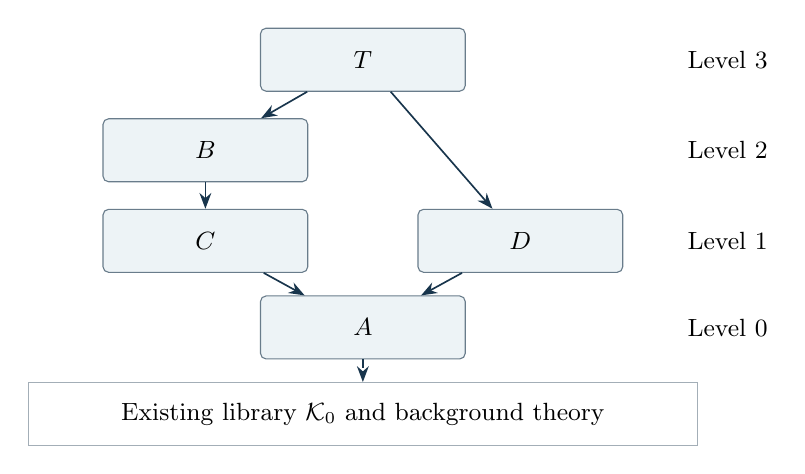
\begin{tikzpicture}[>=Stealth,every node/.style={font=\small},b/.style={draw=ink!65,fill=soft,rounded corners=2pt,minimum width=26mm,minimum height=8mm},a/.style={->,semithick,ink}]
\node[b] (t) at (0,3.4) {$T$};
\node[b] (b) at (-2,2.25) {$B$};
\node[b] (d) at (2,1.1) {$D$};
\node[b] (c) at (-2,1.1) {$C$};
\node[b] (a) at (0,0) {$A$};
\draw[a] (t)--(b);\draw[a] (t)--(d);\draw[a] (b)--(c);\draw[a] (c)--(a);\draw[a] (d)--(a);
\node[anchor=west] at (4.0,3.4) {Level 3};\node[anchor=west] at (4.0,2.25) {Level 2};\node[anchor=west] at (4.0,1.1) {Level 1};\node[anchor=west] at (4.0,0) {Level 0};
\node[draw=ink!40,minimum width=85mm,minimum height=8mm] (k) at (0,-1.1) {Existing library $\K_0$ and background theory};\draw[a,dashed] (a)--(k);
\end{tikzpicture}
\par\small Figure 1. A proof dependency graph with unequal branch depths and a shared lemma. Arrows indicate references; establishment of the results proceeds in the opposite direction.
\end{center}

\begin{proposition}[Uniqueness and strict descent]\label{prop:height}
For a finite directed acyclic graph, equation \eqref{eq:level} uniquely determines the level of every node. The level equals the length, in edges, of the longest dependency path starting at that node. If $v\to u$, then $\ell(u)<\ell(v)$. If all nodes are reachable from $T$, then $T$ is the unique highest-level node.
\end{proposition}
\begin{proof}
Let $h(v)$ be the maximum length of a directed path starting at $v$. The finiteness and acyclicity of the graph guarantee its existence. If $D(v)$ is empty, $h(v)=0$; otherwise every nonempty path first goes to a node in $D(v)$, and $h(v)=1+\max_{u\in D(v)}h(u)$. Hence $h$ satisfies the definition. Induction on $h(v)$ shows that every satisfying assignment agrees with $h$. For each edge, $\ell(v)\ge 1+\ell(u)$. Applying this inequality along any nonempty path from $T$ gives strict descent from the target.
\end{proof}
If $r>0$, repeatedly choosing a dependency attaining the maximum gives a path visiting every level from $r$ to zero. If no new auxiliary lemma is needed, $r=0$; the framework requires no artificial decomposition.

\subsection{Local verification and global correctness}
For each node the local deductive task is
\begin{equation}\label{eq:local}
 \Sigma_0\cup\{P_u:u\in D(v)\}\vdash P_v.
\end{equation}
The researcher examines the inference at this node, including the correct applicability of referenced results, without reconstructing all of the proofs of the already established dependencies.

\begin{proposition}[Compositional correctness]\label{prop:compose}
If \eqref{eq:local} holds at every node, then $\Sigma_0\vdash P_v$ for every $v\in V$. In particular, $\Sigma_0\vdash P_T$.
\end{proposition}
\begin{proof}
Use strong induction on $\ell(v)$. At level zero, there are no new dependencies, and \eqref{eq:local} directly yields $\Sigma_0\vdash P_v$. For a node at level $k>0$, Proposition \ref{prop:height} places every dependency at a lower level. The induction hypothesis gives $\Sigma_0\vdash P_u$ for each $u\in D(v)$. Substituting these derivations into the local proof, or applying the cut principle repeatedly, yields $\Sigma_0\vdash P_v$.
\end{proof}
This is an application of standard logical composition, not a new theorem of proof theory. It establishes the logical consistency of the proposed organization: the validity of all local proofs and their correctly expressed dependencies entails the validity of the target proof. A dependency graph alone is not a proof, and a candidate decomposition need not be valid.

\subsection{Cumulative verification and independent acceptance}
The central institutional change goes beyond organizing a large argument. If every local proof must remain an inseparable part of one paper until the entire project is accepted, the benefit of modular organization is only partially realized. Established local results should be capable of independent assimilation into public mathematical knowledge.

Let $A_t\subseteq V$ denote the nodes whose results have been established along their dependencies and incorporated into shared knowledge after human understanding and verification at time $t$. Write $q_v=(P_v,\pi_v)$ for the proof record. An idealized accumulation is
\begin{equation}\label{eq:library}
 \K_t=\K_0\cup\{q_v:v\in A_t\}.
\end{equation}
In the idealized accumulation model, established records are retained, setting aside corrections and withdrawals: $A_t\subseteq A_{t+1}$. Consequently, $\K_t\subseteq\K_{t+1}$ at each successive stage. The index $t$ denotes a stage of accumulation, not a level of the graph. Local validity with unestablished dependencies is a conditional achievement, not yet an unconditional result relative to $\Sigma_0$.

To describe the distinction precisely, let $Q\subseteq V$ consist of nodes for which the local entailment \eqref{eq:local} has been established. Define the mathematical closure sequence
\[
 C_0=\varnothing,\qquad
 C_{j+1}=C_j\cup\{v\in Q:D(v)\subseteq C_j\}.
\]
Every member of $C_*=\bigcup_{j\ge0} C_j$ is derivable from $\Sigma_0$, by induction on the iteration and composition. The sequence stabilizes because $V$ is finite. It is the least subset of $V$ closed under adjoining nodes in $Q$ whose dependencies already belong to the subset: induction shows that every such closed subset contains each $C_j$.

If $Q=V$, then
\[
 C_j=\{v\in V:\ell(v)<j\},\qquad C_{r+1}=V.
\]
Indeed, the equality holds at $j=0$. A leaf enters at the first iteration; for a non-leaf, all dependencies lie in $C_j$ precisely when their maximum level is less than $j$, equivalent to $\ell(v)\le j$. This proves the equality by induction. These iterations describe logical establishment, not an additional review protocol or a requirement that actual reviewers operate in synchronized rounds.

Mathematicians can begin with the level-zero results, examine their statements and proofs, and add established results to the shared library. An upper-level proof can then directly cite a lower-level result, just as it cites a previously known theorem. It need not reproduce the proof of that result; the original dependency graph provides a path back to its derivation. Independent branches can advance at different rates. The establishment of a node depends on its own dependencies, not on the completion of unrelated branches.

For example, suppose $T$ directly invokes $A$ and $B$, $B$ invokes $C$, and $A,C$ have no new dependencies. The levels are $\ell(A)=\ell(C)=0$, $\ell(B)=1$, and $\ell(T)=2$. Once $A,C$ are established, the remaining local work on $B$ concerns its deduction from $C$ and existing knowledge. After $B$ is established, the target's new local proof can invoke $A,B$ as established results. The direct proof of $T$ can therefore be much shorter than the fully expanded argument, without any loss of access to the latter.

An established lemma can also be valuable before the original target theorem is accepted. It may become an input to a different investigation even if other branches of the original project remain incomplete. In this sense the progress of research can be preserved incrementally rather than expressed solely by success or failure at the target.

The level assignment is relative to the selected graph and its original library boundary $\K_0$. Incorporating a node into $\K_t$ does not invalidate that historical graph. A subsequent investigation can start from $\K_t$, cite the newly available results, and compute levels for its own new proof structure. Thus a proposition has no intrinsic, permanent global level.

\begin{proposition}[Logical conservativity of accumulation]\label{prop:conservative}
If all results recorded in $A_t$ are derivable from $\Sigma_0$, then for every proposition $R$ in the same language,
\[
 \Sigma_0\cup S(\K_t)\vdash R\quad\Longleftrightarrow\quad\Sigma_0\vdash R.
\]
\end{proposition}
\begin{proof}
The reverse implication follows by weakening. In the forward direction a finite derivation uses only finitely many of the newly established statements. Substitute their derivations from $\Sigma_0$ into the proof to obtain a derivation of $R$ from $\Sigma_0$.
\end{proof}
The library enlarges the body of directly accessible, established mathematics; it does not thereby add independent axioms. The model assumes correct records and a fixed background theory. Corrections or withdrawals of erroneous records remain possible in practice, as in ordinary mathematics.

\subsection{Formal correctness, semantic fidelity, and human understanding}
A proof checker establishes a derivation of a specified formal statement. Semantic fidelity concerns whether that statement expresses the intended mathematics. Understanding also encompasses the motivations, mathematical ideas, scope, and relationships of the argument. None of these three notions can simply be identified with another.

When a local proof is accompanied by both mathematical prose and a formal statement, the researcher can examine its objects, quantifiers, hypotheses, conclusion, definitions, and cited results at that local level. A previously examined statement can be reused as an interface for subsequent work. This offers a more tractable organization of semantic assessment than a single enormous translation.

Nevertheless, shortness does not imply simplicity or correctness. A short proof may use sophisticated definitions, and a machine-checked proof of boundedness of continuous functions on $[0,1]$ does not establish boundedness on $(0,1)$, as $f(x)=1/x$ illustrates. The proposed benefit is a reduction in the scope of individual review tasks when decomposition is appropriate, not an automatic guarantee of semantic fidelity. Formal verification tools can assist the process without being the exclusive means of mathematical validation.

\section{Worked example: cross-level citation and reuse}
Consider a real inner product space $H$ with $\|x\|=\sqrt{\langle x,x\rangle}$. For illustration, suppose the initial library contains elementary inner product properties, real arithmetic, and elementary limit laws, but not the following three auxiliary proof records. These are classical results, not new historical discoveries. The target states that if $\|x_n-x\|\to0$ and $\|y_n-y\|\to0$, then $\langle x_n,y_n\rangle\to\langle x,y\rangle$.

\begin{center}
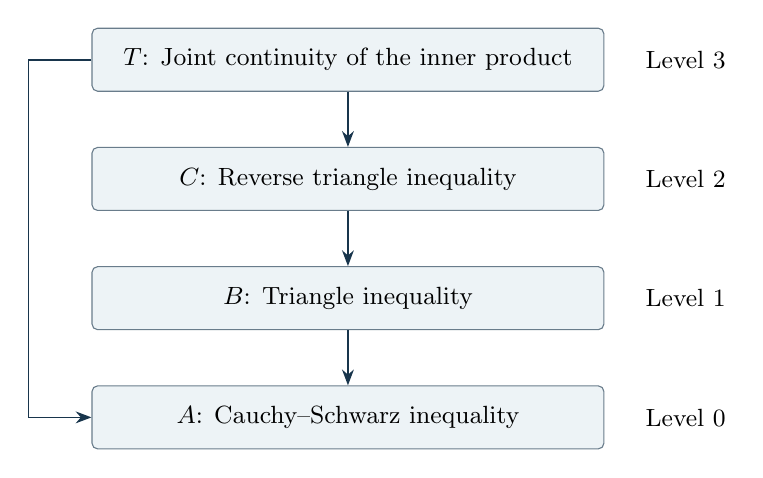
\begin{tikzpicture}[>=Stealth,node distance=7mm,b/.style={draw=ink!65,fill=soft,rounded corners=2pt,minimum width=65mm,minimum height=8mm},every node/.style={font=\small}]
\node[b] (t) {$T$: Joint continuity of the inner product};
\node[b,below=of t] (c) {$C$: Reverse triangle inequality};
\node[b,below=of c] (b) {$B$: Triangle inequality};
\node[b,below=of b] (a) {$A$: Cauchy--Schwarz inequality};
\draw[->,semithick,ink] (t)--(c);\draw[->,semithick,ink] (c)--(b);\draw[->,semithick,ink] (b)--(a);\draw[->,semithick,ink] (t.west)--++(-0.8,0)|-(a.west);
\foreach \n/\k in {t/3,c/2,b/1,a/0}{\node[anchor=west] at ([xshift=4mm]\n.east) {Level \k};}
\end{tikzpicture}
\par\small Figure 2. The target invokes $A$ and $C$; the proof of $B$ also invokes $A$.
\end{center}

\paragraph{Level 0: Lemma $A$ (Cauchy--Schwarz).} For $x,y\in H$, $|\langle x,y\rangle|\le\|x\|\|y\|$.
\begin{proof}
If $y=0$, the conclusion is immediate. Otherwise let $t=\langle x,y\rangle/\|y\|^2$. Positivity and bilinearity give
\[
 0\le\|x-ty\|^2=\|x\|^2-\frac{\langle x,y\rangle^2}{\|y\|^2}.
\]
Rearranging and taking square roots proves the inequality.
\end{proof}
Here $D(A)=\varnothing$, and $\ell(A)=0$.

\paragraph{Level 1: Lemma $B$ (Triangle inequality).} For $x,y\in H$, $\|x+y\|\le\|x\|+\|y\|$.
\begin{proof}
Expanding and applying $A$ gives
\[
 \|x+y\|^2=\|x\|^2+2\langle x,y\rangle+\|y\|^2
 \le(\|x\|+\|y\|)^2.
\]
Taking square roots of the nonnegative quantities yields the desired inequality.
\end{proof}
Thus $D(B)=\{A\}$ and $\ell(B)=1$.

\paragraph{Level 2: Lemma $C$ (Reverse triangle inequality).} For $x,y\in H$, $|\|x\|-\|y\||\le\|x-y\|$.
\begin{proof}
By $B$, $\|x\|\le\|x-y\|+\|y\|$. Interchanging $x,y$ and using $\|y-x\|=\|x-y\|$ gives $\|y\|\le\|x-y\|+\|x\|$. Combine these inequalities.
\end{proof}
Thus $D(C)=\{B\}$ and $\ell(C)=2$.

\paragraph{Level 3: Target theorem $T$.}
\begin{proof}
By $C$, $\|y_n\|\to\|y\|$, so $(\|y_n\|)$ is bounded. Bilinearity and $A$ give
\begin{align*}
 |\langle x_n,y_n\rangle-\langle x,y\rangle|
 &\le |\langle x_n-x,y_n\rangle|+|\langle x,y_n-y\rangle|\\
 &\le\|x_n-x\|\|y_n\|+\|x\|\|y_n-y\|\to0.
\end{align*}
\end{proof}
Consequently $D(T)=\{A,C\}$ and $r=1+\max(0,2)=3$.
\begin{center}\small
\begin{tabular}{ccll}\toprule
Node&Level&Direct new dependencies&Reusable result\\\midrule
$A$&0&None&Inner product estimate\\
$B$&1&$A$&Triangle inequality\\
$C$&2&$B$&Norm difference estimate\\
$T$&3&$A,C$&Joint continuity\\\bottomrule
\end{tabular}
\end{center}
The proof of $A$ is established once, but is invoked by both $B$ and $T$. If another investigation starts with a library containing $A,B,C$, it can cite them without reconstructing this dependency chain. Its own target can be a level-zero node if it requires no further new lemmas. This small example illustrates the organization, not an empirical demonstration of its efficiency on large AI-generated proofs.

\section{Potential benefits and their conditions}
\subsection{Reducing the scope of individual review}
The total size of a proof and the size of its constituent local arguments are different quantities. An appropriate decomposition gives reviewers the opportunity to focus on a well-defined mathematical task, rather than requiring each reviewer to navigate the entire argument. The resulting interfaces can help identify the genuinely novel estimates, reductions, constructions, and conceptual steps. These can be explained, simplified, or generalized independently. The benefit depends on the mathematical quality of the decomposition; more nodes are not intrinsically better.

\subsection{Distributed verification}
Strict descent implies that two nodes at the same level cannot depend on each other, even indirectly. Independent branches can therefore be investigated in parallel. For an idealized model let $c(v)\ge0$ be the time required for a node's task, with unlimited suitable reviewers, no communication cost, and tasks performed after their dependencies. The earliest completion times satisfy
\[
 F(v)=c(v)+\max_{u\in D(v)}F(u),\qquad\max\varnothing:=0.
\]
The target completion time $F(T)$ is the weighted critical path, while total labor is $\sum_{v\in V}c(v)$. This distinction explains how distributed review may shorten elapsed time even when total effort is unchanged. The model does not establish the availability of expert reviewers or quantify real coordination costs.

\subsection{Turning completed review into reusable knowledge}
Suppose projects use proof record sets $V_1,\ldots,V_m$. Identify only records that can genuinely be reused under compatible assumptions and definitions. If establishing record $v$ has constant cost $c(v)$ and it occurs in $m_v$ projects, then the idealized difference between fully repeated establishment and establishing each record once is
\begin{align*}
 W_{\mathrm{repeat}}-W_{\mathrm{reuse}}
 &=\sum_{i=1}^m\sum_{v\in V_i}c(v)-\sum_{v\in\bigcup_i V_i}c(v)\\
 &=\sum_{v\in\bigcup_i V_i}(m_v-1)c(v)\ge0.
\end{align*}
This is a conditional accounting identity, not a measured saving relative to current mathematics, which already makes extensive use of citations. Real costs include searching, maintenance, verifying applicability, and communicating meanings. The proposed shift seeks to make more of the review of intermediate results persist as shared work rather than disappear into a single project.

Over time, AI systems as well as mathematicians can draw upon the newly established results. The work of assimilating one project can then support the production and understanding of the next.

\subsection{Traceability, continuity, and explanation}
Explicit dependencies can help identify the proofs potentially affected by a discovered error by following edges in the reverse direction. Results without that dependency need not be discarded solely because they belong to the same project, provided their premises remain valid. This is a benefit of traceability, not a guarantee of automated repair.

Mathematicians can build explanations, alternative proofs, and generalizations around identifiable nodes. Papers and lectures remain essential for communicating the overarching ideas. The graph supplies access to the local foundations. The two forms of communication are complementary. The desired outcome is not a greater count of lemmas, but an improved capacity to assimilate mathematics and create further mathematics.

\section{Relation to existing work}
Modular proofs and reuse of mathematical results are longstanding practices. Mathlib demonstrates the feasibility of an open, collaboratively developed formal library \cite{mathlib}; Polymath demonstrates large-scale mathematical collaboration \cite{polymath}. Kontorovich's vision of research in the age of AI explicitly considers dependency graphs, multiple resolutions of understanding, and modular mathematical collaboration \cite{kontorovich}. LeanArchitect connects informal blueprints with formal proof dependencies \cite{architect}. MathCoPilot combines human guidance, decomposed proof plans, Lean verification and a knowledge base \cite{copilot}. The Mathlib Initiative's roadmap also addresses shared formal results and information about trust and provenance \cite{roadmap}.

These contributions are substantive precedents, not merely implementation details. In particular, the overlap with Kontorovich's account of future mathematical communication should be acknowledged. This paper makes no claim that dependency graphs, theorem libraries, modular understanding, or their use in collaborative research originated here. Nor does it establish historical priority for every aspect of the proposed institutional shift.

The specific proposal is to articulate a mechanism of cumulative acceptance: identify the new proof nodes relative to the existing library, define their levels by dependency height, organize human understanding and verification around the local results, and preserve established contributions for reuse even while the original target is incomplete. The objective is to make this mechanism a normal organizing principle of research and publication in the presence of large-scale machine-generated mathematics, using existing tools where appropriate.

This is a position paper supported by a formal framework and worked example, not a report of controlled experiments. Its practical superiority over alternative review arrangements remains a question for the mathematical community to investigate.

\section{A call for action}
The concerns raised in recent declarations about AI and mathematics are serious. This paper shares their concern for human understanding, integrity, and the development of mathematical ideas. It argues for a constructive response: rather than allowing new proof production to overwhelm the channels through which mathematics becomes shared knowledge, begin changing those channels now.

The following are invitations to collaboration, not additional rules of the framework.

\paragraph{Mathematicians and research teams.} Explore hierarchical decomposition in substantial research projects. Examine local arguments through seminars, independent review, and collaboration, and disseminate the useful intermediate results as independently reusable knowledge. Continue to explain the main ideas and their implications.

\paragraph{Theorem libraries and proof-assistant communities.} Build on existing resources for sharing local results, examining their statements, and navigating dependencies. Different tools may coexist; the proposed research paradigm does not depend on a single provider or require its proponent to build a new library and checker.

\paragraph{Universities, journals, and mathematical organizations.} Explore how the independent establishment, interpretation, and integration of new proof contributions can be recognized and made citable. Consider how navigable proof records can complement conventional publication. The quality and importance of mathematical work should not be reduced to a count of nodes or checks.

\paragraph{AI laboratories and research funders.} Invest not only in generating proofs, but in making them understandable and useful to mathematicians. Support accessible proof materials, expert participation in mathematical explanation, and shared infrastructure. Sustainable maintenance and review could be supported through grants, sponsorship, research services, or recognition and remuneration of valuable expert contributions. These are possible institutional arrangements, not prescribed commercial or governance rules.

A natural opportunity is the recently released formal proof of the Riemann hypothesis. Existing explanatory work and formal materials could support collaboration on the major reductions and estimates, progressively identifying and examining local arguments and preserving useful established lemmas for further research. This is an invitation to extend work already under way, not a claim that this paper has reorganized or verified the proof itself.

The community can begin with real projects without waiting for universal agreement or a complete new platform. Studies of readability, verification effort, reuse, and subsequent mathematical discovery can inform which practices deserve wider adoption. The need to investigate such benefits is not a reason to defer the conversation.

\section{Conclusion}
An era of greater proof abundance need not be an era of diminished mathematical understanding. Hierarchical proofs and cumulative verification extend the familiar compositional nature of mathematical reasoning into the organization, acceptance, and reuse of research contributions. Rather than treating a vast new proof solely as a single object to be digested, mathematicians can establish, understand, and accumulate its useful constituent results.

The mathematical community should not be compelled to choose between human understanding and the capabilities of AI. It should shape research practices that allow the two to reinforce each other. The goal is not merely for machines to produce more theorems. It is for humanity to understand more mathematics and, on that foundation, to create more mathematics.

\section*{AI use disclosure}
The proposer supplied the central research concept and objective of paradigm change and selected the bottom-up level definition. OpenAI's ChatGPT assisted with formalization of the framework, logical analysis, literature searching, construction of the mathematical example, drafting, and revision. The human author has approved the revisions to this manuscript and is responsible for its content. AI is not listed as an author.

\clearpage
\begin{thebibliography}{99}\small\setlength{\itemsep}{1pt}\setlength{\parskip}{0pt}
\bibitem{thurston} W. P. Thurston. On Proof and Progress in Mathematics. \emph{Bulletin of the AMS}, 30(2), 161--177, 1994. \url{https://doi.org/10.1090/S0273-0979-1994-00502-6}.
\bibitem{tao} T. Tao. Mathematics in the Age of AI. 2026. \url{https://arxiv.org/abs/2608.16753}.
\bibitem{leiden} Leiden Declaration on Artificial Intelligence and Mathematics. June 2, 2026. \url{https://doi.org/10.5281/zenodo.20302944}; \url{https://leidendeclaration.ai/}.
\bibitem{fields} T. Tao and co-signatories. A Severe Misalignment of AI in Mathematics. September 11, 2026. \url{https://terrytao.wordpress.com/2026/09/11/a-severe-misalignment-of-ai-in-mathematics/}.
\bibitem{alpoge} L. Alpöge. Announcement concerning the Riemann Hypothesis. November 20, 2026. \url{https://alpo.ge/remark.pdf}.
\bibitem{rh} Lean FRO and Mathlib Initiative. Lean Verification of the Riemann Hypothesis. Joint statement, November 21, 2026. \url{https://leanprover-community.github.io/blog/posts/riemann-hypothesis/}.
\bibitem{rubinstein} M. Rubinstein. Alpöge/Claude Proof of the Generalized Riemann Hypothesis. Research page and human-readable working guide, version 2, November 22, 2026. \url{https://www.math.uwaterloo.ca/~mrubinst/alpoge_claude_grh/}.
\bibitem{mathlib} The Mathlib Community. The Lean Mathematical Library. \emph{CPP 2020}. \url{https://arxiv.org/abs/1910.09336}.
\bibitem{kontorovich} A. Kontorovich. The Shape of Math To Come. \emph{Proceedings of the International Congress of Mathematicians 2026}, Vol. 2. \url{https://doi.org/10.1137/25M1806764}; preprint \url{https://arxiv.org/abs/2510.15924}.
\bibitem{architect} T. Zhu, P. Monticone, S. Welleck, and J. Avigad. LeanArchitect: Automating Blueprint Generation for Humans and AI. \emph{ITP 2026}, LIPIcs 382, 25:1--25:16. \url{https://doi.org/10.4230/LIPIcs.ITP.2026.25}.
\bibitem{polymath} T. Gowers and M. Nielsen. Massively Collaborative Mathematics. \emph{Nature}, 461, 879--881, 2009. \url{https://doi.org/10.1038/461879a}.
\bibitem{copilot} J. Zhang et al. MathCoPilot: An Interactive System for Human--AI Symbiotic Paradigm of Mathematical Research. 2026. \url{https://arxiv.org/abs/2607.14582}.
\bibitem{roadmap} Mathlib Initiative. The Mathlib Initiative Roadmap (October 2026--March 2027). \url{https://mathlib-initiative.org/roadmap/}.
\end{thebibliography}
\end{document}
